\chapter{Исследовательская часть}
\section{Технические характеристики}
Тестирование выполнялось на устройстве со следующими техническими характеристиками:
\begin{itemize}
	\item Операционная система Pop!\_OS 22.04 LTS \cite{ubuntu} Linux \cite{linux};
	\item Оперативная память 16 Гбайт;
	\item Процессор AMD® Ryzen 7 2700 eight-core processor × 16 \cite{amd}.
\end{itemize}

Во время тестирования устройство было подключено к блоку питания и не нагружено никакими приложениями, кроме встроенных приложений и системой тестирования.

\section{Формализация объекта и его признака}
\label{formal}

Согласно варианту, признаком, по которому будет производиться поиск объектов, будет являться \textit{содержание спирта} в градусах --- целое число.

Определим следующие термы, соответствующие признаку <<содержание спирта>>:
\begin{enumerate}[label=\arabic*)]
	\item <<Легкий>>;
	\item <<Средний>>;
	\item <<Интересный>>;
	\item <<Высокий>>;
	\item <<Не употребительный>>.
\end{enumerate}


\section{Демонстрация работы программы}


Результат работы программы, в которой выводится время работы алгоритма представлено на рисунке \ref{demonstration}.

\begin{figure}[ht!]
	\begin{center}
		\captionsetup{singlelinecheck = false, justification=centerfirst}
		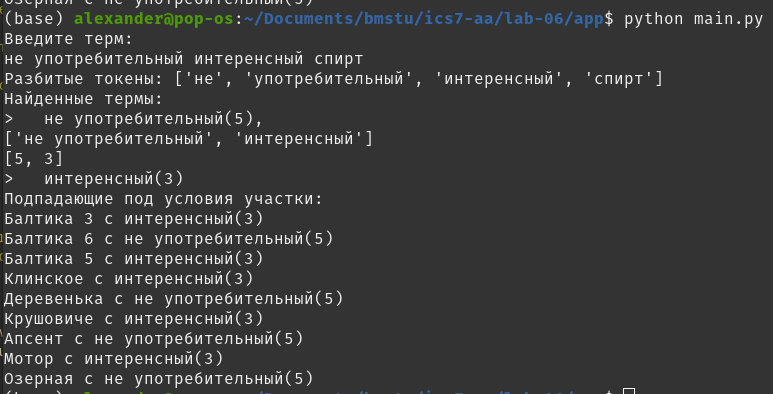
\includegraphics[scale=0.6]{assets/demon.png}
		\caption{Пример работы программы}
		\label{demonstration}
	\end{center}
	
	
\end{figure}

\newpage


\subsection{Построение функции принадлежности термам}

Построим графики функций принадлежности числовых значений переменной термам, описывающим группы значений лингвистической переменной.

Для этого для каждого значения из количества спирта для каждого терма из перечисленных найдём количество респондентов, согласно которым значение удовлетворяет сопоставляемому терму.
Данное значение поделим на количество респондентов --- это и будет значением функции $\mu$ для терма в точке.
Графики функций принадлежности числовых значений роста термам, приведён на рисунке \ref{img:fig1}.

\begin{figure}[ht!]
	\begin{center}
		\captionsetup{singlelinecheck = false, justification=centerfirst}
		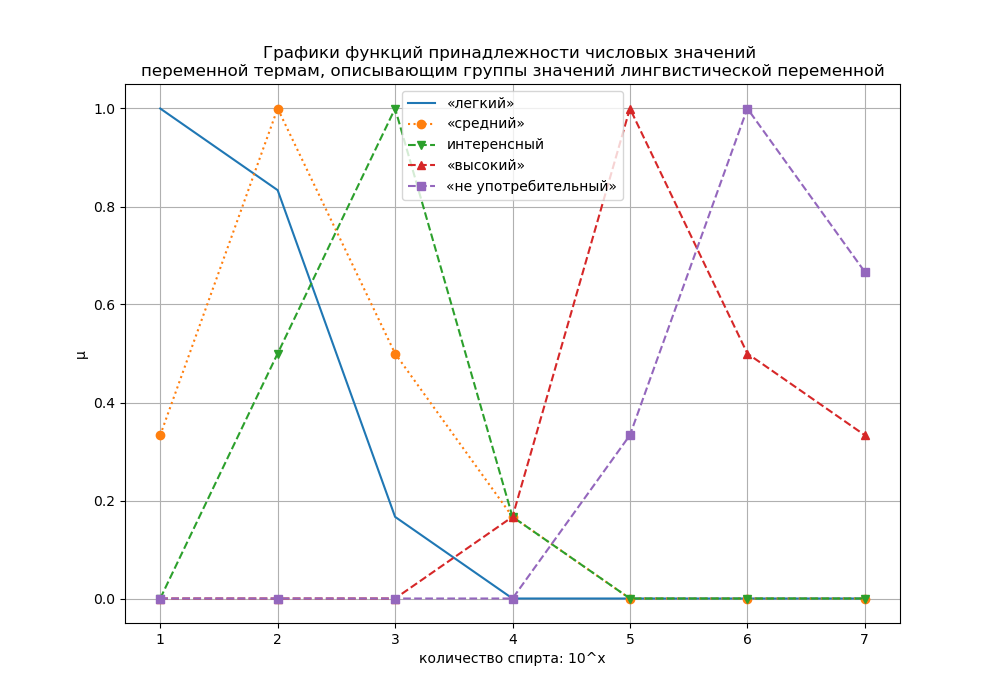
\includegraphics[scale=0.6]{assets/graphs/Figure_1.png}
		\caption{Графики функций принадлежности числовых значений переменной термам}
		\label{img:fig1}
	\end{center}
	
	
\end{figure}